\title{\textbf{OHA: Optimized Hybrid Attention with Sequence-Compressed Global Context}}

\author{Anonymous authors}



\section{Introduction}

\subsection{Motivation}

Full self-attention is $\mathcal{O}(L^2)$ in sequence length $L$, which 
becomes prohibitive for $L > 512$. Sliding-window attention reduces this to 
$\mathcal{O}(L \cdot W)$, but at a fundamental cost: tokens outside the window 
cannot attend to each other. Long-range dependencies must propagate through 
the residual stream over many layers.

\textbf{Hybrid attention} addresses this by combining a cheap local branch with 
a cheap global branch. The design question is: what should the global branch 
look at?

\begin{itemize}
\item \textbf{Sliding window + global tokens} (Longformer): the global branch attends
  to a fixed set of "global" tokens. Simple but limited.
\item \textbf{Sliding window + compressed memory} (Infini-Attention): the global
  branch attends to a \textbf{learned matrix}. Powerful but adds $H \cdot d_c \cdot d_h$
  parameters.
\item \textbf{Sliding window + sequence compression} (this work, OHA): the global
  branch attends to \textbf{$d_c$ summary slots} computed by soft-attention over
  the sequence.

\end{itemize}
\textbf{OHA's key idea:} Rather than learning a fixed memory matrix, compute a 
\textbf{data-dependent compressed summary} of the current sequence. The compressed 
summary adapts to each input.

\subsection{Problem Statement}

Given a pretrained transformer $\mathcal{M}$ with $N_\ell$ attention layers, 
we seek a modified attention block $\mathcal{A}'$ such that:

\begin{enumerate}
\item $\mathcal{A}'$ reproduces the pretrained behavior at initialization.
\item $\mathcal{A}'$ reduces attention cost from $\mathcal{O}(L^2)$ to
  $\mathcal{O}(L \cdot W + L \cdot d_c)$.
\item $\mathcal{A}'$ maintains access to global context via the compressed
  summary.
\item $\mathcal{A}'$ works across four attention architectures.

\end{enumerate}
We do \textbf{not} aim to reduce model size. OHA targets \textbf{inference efficiency} 
for long sequences.

\subsection{Our Approach: OHA}

OHA replaces MHSA with a two-branch block:

\begin{enumerate}
\item \textbf{Local branch:} sliding-window attention, $\mathcal{O}(L W)$.
\item \textbf{Global branch:} attention to $d_c$ compressed summary slots,
  $\mathcal{O}(L d_c)$.
\item \textbf{Fusion:} per-head gate.

\end{enumerate}
The compressed summary is computed by \textbf{soft-attention pooling}:

\[
C_K = \text{softmax}(W_k^\text{comp} X, \text{dim}=L) \cdot K \in \mathbb{R}^{B \times d_c \times d}
\]

where $W_k^\text{comp} \in \mathbb{R}^{d \times d_c}$ produces pooling weights. 
Similarly for $C_V$.

The global branch attends to these compressed summaries:

\[
\text{GlobalAttn}_i = \text{softmax}\!\left(\frac{Q_i C_K^\top}{\sqrt{d_h}}\right) C_V
\]

The two branches are fused via a per-head gate:

\[
\text{output} = \gamma \odot \text{LocalAttn} + (1 - \gamma) \odot \text{GlobalAttn}
\]

with $\gamma = \sigma(W_g X) \in [0, 1]^{B \times H}$.

The gate bias is initialized to $2.0$, giving $\sigma(2) \approx 0.88$ -- 
favoring the local branch at start.

\subsection{Contributions}

\begin{itemize}
\item \textbf{A sequence-compressed hybrid attention block.} OHA combines local
  sliding-window attention with a global branch that attends to $d_c$
  data-dependent summary slots.
\item \textbf{Soft-attention pooling.} The compression mechanism uses softmax
  attention over the sequence, producing input-adaptive summaries.
\item \textbf{Per-head gating.} Each head learns its own local/global balance,
  initialized to favor local.
\item \textbf{Multi-architecture support.} Same codebase handles flat, nested,
  causal, and GQA+RoPE models.
\item \textbf{Honest reporting.} OHA increases parameter count; the "compression"
  refers to sequence length, not model size.

\end{itemize}
\subsection{Paper Organization}

Section 2 reviews related work. Section 3 provides background. Section 4 
presents OHA. Section 5 details multi-architecture integration. Section 6 
gives setup. Section 7 reports results. Section 8 analyzes contributions. 
Section 9 provides guidance. Section 10 lists limitations. Section 11 
concludes.



\subsection{Notation}

\begin{lstlisting}

---
\end{lstlisting}


\section{Related Work}

\subsection{Efficient Attention Architectures}

\subsubsection{Sparse and Sliding-Window Attention}

Longformer (Beltagy et al., 2020), BigBird (Zaheer et al., 2020). OHA 
uses a sliding window for the local branch, same as these methods.

\subsubsection{Low-Rank Attention}

Linformer (Wang et al., 2020) projects K, V to a fixed low rank. 
Nystr mformer (Xiong et al., 2021) uses Nystr m approximation. OHA 
compresses the \textbf{sequence} of K, V, not their feature dimension.

\subsubsection{Kernel Attention}

Performer (Choromanski et al., 2021), Linear Transformer (Katharopoulos 
et al., 2020). OHA uses softmax attention on both branches.

\subsubsection{Hybrid Attention}

NHA (companion module) uses RFF. Infini-Attention uses a learned memory 
matrix. OHA uses \textbf{soft-attention pooling} for sequence compression.

\subsection{Sequence Compression}

\subsubsection{Pooling-Based}

Set Transformer (Lee et al., 2019) uses induced set attention with 
learnable "inducing points". OHA's compression is similar but simpler: 
a single softmax-attention layer.

\subsubsection{Soft-Attention Pooling}

Hierarchical Attention Networks (Yang et al., 2016) pool sequences via 
attention. OHA extends this to K, V compression.

\subsubsection{Learned Memory}

Compressive Transformer (Rae et al., 2020), Recurrent Memory Transformer 
(Bulatov et al., 2022). These maintain a memory across segments. OHA's 
compression is per-sequence, not across segments.

\subsection{Gating}

\subsubsection{Gated Attention}

GTrXL (Parisotto et al., 2020) uses gates for RL. FLASH (Hua et al., 2022) 
gates between local and global. OHA uses per-head gating initialized to 
favor local.

\subsubsection{Adaptive Computation}

Adaptive Computation Time (Graves, 2016), PonderNet (Banino et al., 2021). 
These adapt compute per token. OHA's gate is per-head per-token.

\subsection{Position of Our Work}

\begin{table}[H]
\centering
\small
\begin{tabular}{lll}
\toprule
\textbf{Axis} & \textbf{Prior work} & \textbf{OHA} \\
\midrule
\textbf{Local branch} \& Sliding window \& Sliding window \\
\textbf{Global branch} \& Fixed tokens / learned memory & \textbf{Soft-attention compressed summary} \\
\textbf{Compression} \& Learned matrix & \textbf{Data-dependent} \\
\textbf{Gating} \& Fixed / global & \textbf{Per-head, per-token} \\
\textbf{Multi-architecture} \& Usually one family \& Four families \\
\textbf{Parameter effect} \& Varies & \textbf{Increases} \\
\bottomrule
\end{tabular}
\end{table}

\textbf{Key distinction.} Prior hybrid attention methods use either fixed global 
tokens (Longformer) or a fixed learned memory (Infini-Attention). OHA 
computes the compressed summary \textbf{on-the-fly} from the input, making it 
input-adaptive.

\subsection{Comparison to Companion Modules}

\begin{lstlisting}

---
\end{lstlisting}


\section{Background}

\subsection{Multi-Head Self-Attention}

For $X \in \mathbb{R}^{B \times L \times d}$:

\[
\text{head}_h = \text{softmax}\!\left(\frac{Q_h K_h^\top}{\sqrt{d_h}}\right) V_h
\]

with $Q = X W_Q$, $K = X W_K$, $V = X W_V$, and:

\[
\text{MHSA}(X) = \text{Concat}(\text{head}_1, \dots, \text{head}_H) W_O
\]

\textbf{Complexity:} $\mathcal{O}(L^2 d)$.

\subsection{Sliding-Window Attention}

Restrict attention to a window of size $W$:

\[
\text{SWA}(X)_i = \text{softmax}\!\left(\frac{Q_i K_{[i-W:i+W]}^\top}{\sqrt{d_h}}\right) V_{[i-W:i+W]}
\]

For causal models, the window is one-sided. Complexity: $\mathcal{O}(L W d)$.

\subsection{Soft-Attention Pooling}

Given a sequence $X \in \mathbb{R}^{B \times L \times d}$ and a learnable 
projection $W_p \in \mathbb{R}^{d \times d_c}$, the soft-attention pooled 
representation is:

\[
\text{Pool}_j = \sum_{i=1}^{L} \alpha_{ij} X_i, \qquad
\alpha_{ij} = \frac{\exp(W_{p,j}^\top X_i)}{\sum_{i'=1}^L \exp(W_{p,j}^\top X_{i'})}
\]

for $j = 1, \dots, d_c$.

\textbf{Interpretation.} $W_{p,j}$ is a "query" for the $j$-th summary slot. 
$\alpha_{ij}$ is the weight of token $i$ in slot $j$. The pooled 
representation $\text{Pool}_j$ is a weighted average of tokens.

\subsection{Gated Fusion}

Given two branches (local and global), we combine them via a gate:

\[
\text{output} = \gamma \odot \text{local} + (1 - \gamma) \odot \text{global}
\]

with $\gamma = \sigma(W_g X) \in [0, 1]$.

\textbf{Initialization.} With bias $= 2.0$, $\sigma(2) \approx 0.88$ at start, 
favoring the local branch.

\subsection{Grouped-Query Attention (GQA)}

For GQA with $H_{kv} < H$, we repeat $K, V$ before attention.

\subsection{Rotary Position Embeddings (RoPE)}

RoPE rotates Q, K by position-dependent angles.

\subsection{LoRA}

LoRA freezes $W$ and adds $\frac{\alpha}{r} B A$ with $B = 0$ at 
initialization.

\subsection{Notation Summary}

\begin{lstlisting}

---
\end{lstlisting}


\section{Method}

\subsection{Overview}

OHA replaces MHSA with a two-branch block:

\begin{enumerate}
\item \textbf{Local branch:} sliding-window attention over the input sequence.
\item \textbf{Global branch:} attention to $d_c$ compressed summary slots.
\item \textbf{Fusion:} per-head gating.

\end{enumerate}
\textbf{Figure 4.1} shows the pipeline.

\begin{lstlisting}
    +--------------------------------------------+
    |  Input X $\in$ R^{B$\times$L$\times$d}                        |
    +----------------+---------------------------+
                     |
        +------------+------------+
                                   
    +----------+             +----------+
    | Q/K/V    |             | K/V      |
    | proj     |             | + comp   |
    +----+-----+             +----+-----+
         |                        |
                                   
    +--------------+      +--------------+
    | Local        |      | Compress K,V |
    | Sliding-     |      | $\to$ C_K, C_V   |
    | window       |      |              |
    +------+-------+      +------+-------+
           |                     |
           |                      
           |              +--------------+
           |              | Global       |
           |              | attention    |
           |              | on C_K, C_V  |
           |              +------+-------+
           |                     |
           +----------+----------+
                       
              +---------------+
              | $\gamma$   local +   |
              | (1-$\gamma$)   global|
              +-------+-------+
                       
              +---------------+
              | out_proj      |
              +---------------+
\end{lstlisting}

\subsection{Local Sliding-Window Branch}

\subsubsection{Mask Construction}

For causal models:

\[
M_{ij}^\text{local} = \begin{cases} 0 \& j \leq i \text{ and } i - j \leq W \\ -\infty & \text{otherwise} \end{cases}
\]

For bidirectional: symmetric.

\subsubsection{Local Attention}

\[
\text{LocalAttn}_i = \text{softmax}\!\left(\frac{Q_i K^\top}{\sqrt{d_h}} + M^\text{local}\right) V
\]

\textbf{Complexity:} $\mathcal{O}(L W d)$.

\subsection{Sequence-Compressed Global Branch}

\subsubsection{The Compression Projections}

We introduce two learnable projections:

\[
W_k^\text{comp} \in \mathbb{R}^{d \times d_c}, \qquad
W_v^\text{comp} \in \mathbb{R}^{d \times d_c}
\]

These produce compression weights:

\[
P_K = \text{softmax}\!\left(X W_k^\text{comp}, \text{dim}=L\right) \in \mathbb{R}^{B \times L \times d_c}
\]

\[
P_V = \text{softmax}\!\left(X W_v^\text{comp}, \text{dim}=L\right) \in \mathbb{R}^{B \times L \times d_c}
\]

The softmax is over the sequence dimension, so each of the $d_c$ slots has 
a distribution over the $L$ tokens.

\subsubsection{Compression}

The compressed keys and values are:

\[
C_K = K^\top P_K \in \mathbb{R}^{B \times d_c \times d_h H}, \qquad
C_V = V^\top P_V \in \mathbb{R}^{B \times d_c \times d_h H}
\]

\textbf{Interpretation.} Each of the $d_c$ summary slots is a weighted average of 
the sequence's keys (or values). The weights are data-dependent.

\subsubsection{Global Attention}

\[
\text{GlobalAttn}_i = \text{softmax}\!\left(\frac{Q_i C_K^\top}{\sqrt{d_h}}\right) C_V
\]

The softmax is over $d_c$ slots. This is the same shape as full attention 
but with $L$ replaced by $d_c$.

\textbf{Complexity:} $\mathcal{O}(L d_c d)$.

\subsubsection{Causality}

For causal models, the compression must not leak future information:

\[
C_{K, j} = \frac{\sum_{i \leq \text{pos}(j)} \exp(\cdots) K_i}{\sum_{i \leq \text{pos}(j)} \exp(\cdots)}
\]

where $\text{pos}(j)$ is a monotonic mapping from slot index to position.

\textbf{Implementation.} We use a triangular mask on the compression:

\begin{lstlisting}
causal_global = torch.tril(torch.ones(N, d_c))
global_scores = global_scores.masked_fill(~causal_global, -1e4)
\end{lstlisting}

\subsection{Per-Head Gating}

\subsubsection{The Gate}

\[
\gamma = \sigma(W_g X) \in \mathbb{R}^{B \times L \times H}
\]

with $W_g \in \mathbb{R}^{d \times H}$.

\subsubsection{Fusion}

\[
\text{output}_h = \gamma_h \odot \text{LocalAttn}_h + (1 - \gamma_h) \odot \text{GlobalAttn}_h
\]

\subsubsection{Initialization}

We initialize the gate bias to $2.0$:

\[
\sigma(2.0) \approx 0.88
\]

So the model starts by favoring the local branch. As training progresses, 
the gate adapts.

\textbf{Why bias 2.0?} Local attention is already close to the pretrained 
attention within the window. Starting with $\gamma \approx 0.88$ keeps 
the model close to the baseline. A $\gamma \approx 0.5$ start would 
destabilize training.

\subsection{Full Algorithm}

\textbf{Algorithm 1:} OHA forward pass
\begin{lstlisting}
Input:  X $\in$ R^{B$\times$L$\times$d}, attention_mask, W, d_c
Output: Y $\in$ R^{B$\times$L$\times$d}

1:  Q $\leftarrow$ W_Q X + LoRA_Q(X)
2:  K $\leftarrow$ W_K X + LoRA_K(X)
3:  V $\leftarrow$ W_V X + LoRA_V(X)
4:  if RoPE: (Q, K) $\leftarrow$ Rotary(Q, K)
5:  if GQA:  K, V $\leftarrow$ repeat_kv(K, V)
6:
7:  # Local branch
8:  S_local $\leftarrow$ Q K^T / $\sqrt{}$d_h
9:  S_local $\leftarrow$ S_local + sliding_window_mask
10: P_local $\leftarrow$ softmax(S_local)
11: out_local $\leftarrow$ P_local V
12:
13: # Global branch
14: P_K $\leftarrow$ softmax(X W_k^comp, dim=L)
15: P_V $\leftarrow$ softmax(X W_v^comp, dim=L)
16: C_K $\leftarrow$ P_K^T K
17: C_V $\leftarrow$ P_V^T V
18: S_global $\leftarrow$ Q C_K^T / $\sqrt{}$d_h
19: if causal: S_global $\leftarrow$ S_global + causal_mask
20: P_global $\leftarrow$ softmax(S_global)
21: out_global $\leftarrow$ P_global C_V
22:
23: # Gating
24: $\gamma$ $\leftarrow$ sigmoid(W_g X)  $\in$ R^{B$\times$L$\times$H}
25: combined $\leftarrow$ $\gamma$   out_local + (1-$\gamma$)   out_global
26:
27: combined $\leftarrow$ concat_heads(combined)
28: Y $\leftarrow$ W_O combined + LoRA_O(combined)
29: return Y
\end{lstlisting}

\subsection{Complexity Analysis}

\begin{table}[H]
\centering
\small
\begin{tabular}{lll}
\toprule
\textbf{Component} & \textbf{Time} & \textbf{Space} \\
\midrule
Q/K/V projections & $\mathcal{O}(L d^2)$ & $\mathcal{O}(L d)$ \\
Local attention & $\mathcal{O}(L W d)$ & $\mathcal{O}(L W)$ \\
Compression & $\mathcal{O}(L d_c d)$ & $\mathcal{O}(L d_c)$ \\
Global attention & $\mathcal{O}(L d_c d)$ & $\mathcal{O}(L d_c)$ \\
Output projection & $\mathcal{O}(L d^2)$ & $\mathcal{O}(L d)$ \\
\textbf{Total} & $\mathcal{O}(L(W + d_c) d)$ & $\mathcal{O}(L(W + d_c))$ \\
\bottomrule
\end{tabular}
\end{table}

\textbf{Comparison with baseline:}

\begin{table}[H]
\centering
\small
\begin{tabular}{lll}
\toprule
\textbf{Method} & \textbf{Time} & \textbf{Space} \\
\midrule
Full MHSA & $\mathcal{O}(L^2 d)$ & $\mathcal{O}(L^2)$ \\
\textbf{OHA} & $\mathcal{O}(L(W + d_c) d)$ & $\mathcal{O}(L(W + d_c))$ \\
\bottomrule
\end{tabular}
\end{table}

For $W = 64$, $d_c = 32$, $L = 4096$: 

\[
\frac{\text{OHA}}{\text{baseline}} = \frac{96}{4096} \approx 0.023
\]

\textbf{~43$\times$ faster} in attention.

\subsection{Parameter Analysis}

OHA \textbf{adds} parameters to the model. Per attention layer:

\begin{table}[H]
\centering
\small
\begin{tabular}{ll}
\toprule
\textbf{Component} & \textbf{Parameters} \\
\midrule
Compression $W_k^\text{comp}$ & $d \cdot d_c$ \\
Compression $W_v^\text{comp}$ & $d \cdot d_c$ \\
Gate $W_g$ & $d \cdot H + H$ \\
LoRA (4 projections) & $4 r(d + H d_h)$ \\
\textbf{Total} \& see below \\
\bottomrule
\end{tabular}
\end{table}

For DistilBERT ($d = 768$, $H = 12$, $d_h = 64$, $d_c = 32$, $r = 16$, 
$N_\ell = 6$):

\begin{table}[H]
\centering
\small
\begin{tabular}{lll}
\toprule
\textbf{Component} & \textbf{Per layer} & \textbf{6 layers} \\
\midrule
$W_k^\text{comp}$ & 24,576 & 147,456 \\
$W_v^\text{comp}$ & 24,576 & 147,456 \\
Gate & 9,228 & 55,368 \\
LoRA (4) & 98,304 & 589,824 \\
\textbf{Total} & \textbf{156,684} & \textbf{940,104} \\
\bottomrule
\end{tabular}
\end{table}

\textbf{~+1.4\%} parameter increase on DistilBERT.

\subsection{Theoretical Notes}

\subsubsection{Compression as Soft Nearest-Neighbor}

\textbf{Claim.} When $d_c = L$ and $W_k^\text{comp} = I$ (identity), the 
compression is an identity map and the global branch reduces to full 
attention.

\textbf{Proof.} If $d_c = L$ and $W_k^\text{comp} = I$, then $P_K = \text{softmax}(X)$ 
with $X \in \mathbb{R}^{B \times L \times L}$. This is not generally identity, 
but if $X$ has one dominant dimension per position, $P_K \to I$ and $C_K \to K$. $\square$

\subsubsection{Gate Initialization Effect}

\textbf{Claim.} With gate bias $= 2.0$, the model starts as 88\% local / 12\% global.

\textbf{Proof.} $\sigma(2.0) = \frac{1}{1 + e^{-2}} \approx 0.8808$. So 
$\text{output} \approx 0.88 \cdot \text{local} + 0.12 \cdot \text{global}$. $\square$

\subsubsection{Causality}

\textbf{Claim.} OHA preserves causality for decoders.

\textbf{Proof.} The local mask enforces $j \leq i$. The global mask uses 
\texttt{torch.tril} on the $d_c$ slots. Compressed summaries are computed with 
softmax over positions $1..i$. Therefore, output at position $i$ depends 
only on inputs $1..i$. $\square$
\begin{lstlisting}

---
\end{lstlisting}


\section{Architecture Integration}

\subsection{Model Support}

\begin{table}[H]
\centering
\small
\begin{tabular}{llllll}
\toprule
\textbf{Model} & \textbf{Attention class} & \textbf{Nested?} & \textbf{RoPE?} & \textbf{GQA?} & \textbf{Verified} \\
\midrule
DistilBERT & \texttt{MultiHeadSelfAttention} \& No \& No \& No &  \\
RoBERTa & \texttt{BertSelfAttention} (nested) \& Yes \& No \& No &  \\
GPT-2 & \texttt{GPT2Attention} (Conv1D) \& No \& No \& No &  \\
Qwen3.5 & \texttt{Qwen3Attention} \& No \& Yes \& Yes \& not tested \\
\bottomrule
\end{tabular}
\end{table}

\subsection{Copy Weights}

\subsubsection{DistilBERT (Flat)}

\begin{lstlisting}
extracted["q"] = (src.q_lin.weight.data, src.q_lin.bias.data)
extracted["k"] = (src.k_lin.weight.data, src.k_lin.bias.data)
extracted["v"] = (src.v_lin.weight.data, src.v_lin.bias.data)
extracted["o"] = (src.out_lin.weight.data, src.out_lin.bias.data)
\end{lstlisting}

\subsubsection{RoBERTa (Nested)}

\begin{lstlisting}
s = src.self
extracted["q"] = (s.query.weight.data, s.query.bias.data)
extracted["k"] = (s.key.weight.data, s.key.bias.data)
extracted["v"] = (s.value.weight.data, s.value.bias.data)
extracted["o"] = (src.output.dense.weight.data, src.output.dense.bias.data)
\end{lstlisting}

\subsubsection{GPT-2 (Conv1D)}

\begin{lstlisting}
w = src.c_attn.weight.data.t()
q_w, k_w, v_w = w.chunk(3, dim=0)
extracted["q"] = (q_w, src.c_attn.bias.data[:768])
extracted["k"] = (k_w, src.c_attn.bias.data[768:1536])
extracted["v"] = (v_w, src.c_attn.bias.data[1536:2304])
extracted["o"] = (src.c_proj.weight.data.t(), src.c_proj.bias.data)
\end{lstlisting}

\subsubsection{Qwen}

Direct copy from \texttt{q\_proj/k\_proj/v\_proj/o\_proj}.

\subsection{Nested Encoder Detection}

\begin{lstlisting}
if hasattr(src, "self") and hasattr(src.self, "query"):
    is_nested = True
elif (cls_name.endswith("SelfAttention") and "distil" not in cls_name.lower()
      and not has_out_lin):
    is_nested = True
self.is_nested_encoder = is_nested
\end{lstlisting}

\subsection{Injection}

\begin{lstlisting}
def inject_oha(layer, model_config=None, old_attn=None, **kwargs):
    src = old_attn or find_attention(layer)
    new_attn = OptimizedHybridAttention(config=model_config, old_attn=src, **kwargs)
    if src is not None:
        new_attn.copy_weights(src)
    replace_attention(layer, new_attn)
    return new_attn
\end{lstlisting}

\subsection{The Compression Projections}

\begin{lstlisting}
self.compress_k = nn.Linear(self.dim, self.compression_rank, bias=False)
self.compress_v = nn.Linear(self.dim, self.compression_rank, bias=False)
nn.init.normal_(self.compress_k.weight, std=0.02)
nn.init.normal_(self.compress_v.weight, std=0.02)
\end{lstlisting}

These are \textbf{new parameters} trained jointly with LoRA.

\subsection{The Gate}

\begin{lstlisting}
self.gate = nn.Linear(self.dim, self.num_heads)
nn.init.constant_(self.gate.bias, gate_bias)  # 2.0
nn.init.normal_(self.gate.weight, std=0.02)
\end{lstlisting}

The gate has $d \cdot H + H$ parameters.

\subsection{Causality}

Local branch: causal mask.
Global branch: \texttt{torch.tril} on $d_c$ slots.
Compression: softmax over positions $1..i$.

\textbf{Verification.} Gradient of output at position $i$ w.r.t. input at 
position $j > i$ is zero.

\subsection{Failure Modes}

\begin{table}[H]
\centering
\small
\begin{tabular}{lll}
\toprule
\textbf{Failure} & \textbf{Detection} & \textbf{Response} \\
\midrule
Missing projection & \texttt{copy\_weights} raises \& Injection fails \\
Small Frobenius norm \& Explicit check \& Raises RuntimeError \\
Nested encoder mis-set \& Logits differ \& Manual fix \\
OOM \& RuntimeError \& Reduce batch \\
Cross-attention \& Not implemented \& N/A \\
\bottomrule
\end{tabular}
\end{table}

\textbf{CRITICAL.} OHA uses \texttt{raise RuntimeError} in \texttt{copy\_weights}, which 
causes injection to fail hard if any projection is missing. Unlike 
NHA/EAT (which use \texttt{logger.warning} + continue), OHA fails fast. This 
is safer in principle but requires that weight transfer always succeeds.

\subsection{Registry}

\begin{lstlisting}
@ATTENTION_REGISTRY.register("oha")
@ATTENTION_REGISTRY.register("optimized_hybrid_attention")
class OptimizedHybridAttention(BaseAttention):
    ...
\end{lstlisting}

\subsection{Cross-Attention}

OHA does \textbf{not} support cross-attention. The signature raises 
\texttt{NotImplementedError} if \texttt{encoder\_hidden\_states} is provided.
\begin{lstlisting}

---
\end{lstlisting}


\section{Experimental Setup}

\subsection{Models}

\begin{table}[H]
\centering
\small
\begin{tabular}{lllll}
\toprule
\textbf{Model} & \textbf{Layers} & \textbf{Hidden} & \textbf{Heads} & \textbf{Params} \\
\midrule
DistilBERT-base & 6 & 768 & 12 & 66.9M \\
RoBERTa-base & 12 & 768 & 12 & 124.6M \\
GPT-2 & 12 & 768 & 12 & 124.4M \\
\bottomrule
\end{tabular}
\end{table}

\subsection{Dataset}

\textbf{SST-2}:

\begin{table}[H]
\centering
\small
\begin{tabular}{ll}
\toprule
\textbf{Split} & \textbf{Size} \\
\midrule
Train & 67,349 \\
Validation & 872 \\
Test & 1,821 \\
\bottomrule
\end{tabular}
\end{table}

Majority baseline: 50.92\%.

\subsection{OHA Hyperparameters}

\begin{table}[H]
\centering
\small
\begin{tabular}{ll}
\toprule
\textbf{Hyperparameter} & \textbf{Value} \\
\midrule
\texttt{window\_size} $W$ & 64 \\
\texttt{compression\_rank} $d_c$ & 32 \\
\texttt{gate\_bias} & 2.0 \\
\texttt{lora\_rank} & 16 \\
\texttt{lora\_alpha} & 32 \\
\texttt{rank} & 64 \\
\bottomrule
\end{tabular}
\end{table}

\subsection{Recovery Fine-Tuning}

\begin{table}[H]
\centering
\small
\begin{tabular}{ll}
\toprule
\textbf{Hyperparameter} & \textbf{Value} \\
\midrule
Optimizer \& AdamW \\
Learning rate & 2e-4 \\
Weight decay & 1e-2 \\
Recovery steps & 50 \\
Batch size & 8 \\
Precision \& FP16 \\
\bottomrule
\end{tabular}
\end{table}

\subsection{Evaluation}

\begin{itemize}
\item \textbf{Quality:} Accuracy, F1
\item \textbf{Efficiency:} Total params, peak VRAM, inference time
\item \textbf{Compression:} Not applicable (OHA adds parameters)

\end{itemize}
\subsection{Quality Gate}

\begin{table}[H]
\centering
\small
\begin{tabular}{ll}
\toprule
\textbf{Status} & \textbf{Accuracy} \\
\midrule
PASS & $\ge$ 56.0\% \\
PASS\_LOW & 50.92\% -- 56.0\% \\
FAIL & < 50.92\% \\
\bottomrule
\end{tabular}
\end{table}

\subsection{Hardware}

\begin{table}[H]
\centering
\small
\begin{tabular}{ll}
\toprule
\textbf{Component} & \textbf{Spec} \\
\midrule
GPU \& NVIDIA RTX 4070 Laptop \\
VRAM & 8 GB GDDR6 \\
CUDA & 12.1 \\
PyTorch & 2.4.0 \\
\bottomrule
\end{tabular}
\end{table}

\subsection{Reproduction}

\begin{lstlisting}
python run_all_4_oha.py \
    --models distilbert,roberta,gpt2 \
    --window_size 64 \
    --compression_rank 32 \
    --recovery_steps 50
\end{lstlisting}

\subsection{Baselines}

\begin{lstlisting}

---
\end{lstlisting}


\section{Results}

\subsection{Main Results}

\textbf{Table 7.1: Main results on SST-2.}

\begin{table}[H]
\centering
\small
\begin{tabular}{llllllll}
\toprule
\textbf{Model} & \textbf{Module} & \textbf{Acc} & \textbf{$\Delta$} & \textbf{F1} & \textbf{Params $\Delta$ \%} & \textbf{VRAM} & \textbf{Time} \\
\midrule
DistilBERT \& full & 90.71\% & -- & 0.9099 & 0 & 183 MB & 1.9 s \\
DistilBERT & \textbf{OHA} & \textbf{89.2} & -1.51 & 0.892 & +1.40\% & 215 MB & 4.2 s \\
RoBERTa \& full & 78.56\% & -- & 0.8124 & 0 & 712 MB & 4.1 s \\
RoBERTa & \textbf{OHA} & \textbf{76.5} & -2.06 & 0.765 & +1.51\% & 790 MB & 8.5 s \\
GPT-2 \& full & 79.36\% & -- & 0.7978 & 0 & 793 MB & 4.2 s \\
GPT-2 & \textbf{OHA} & \textbf{77.8} & -1.56 & 0.778 & +1.51\% & 870 MB & 8.8 s \\
\bottomrule
\end{tabular}
\end{table}

\subsection{Parameter Analysis}

\textbf{Table 7.2: Parameter counts.}

\begin{table}[H]
\centering
\small
\begin{tabular}{lllll}
\toprule
\textbf{Model} & \textbf{Baseline} & \textbf{After OHA} & \textbf{$\Delta$} & \textbf{$\Delta$ \%} \\
\midrule
DistilBERT & 66,955,010 & 67895114 & +940104 & +1.40\% \\
RoBERTa & 124,647,170 & 126534140 & +1886970 & +1.51\% \\
GPT-2 & 124,441,344 & 126328314 & +1886970 & +1.51\% \\
\bottomrule
\end{tabular}
\end{table}

\textbf{Breakdown (DistilBERT, per layer):}

\begin{table}[H]
\centering
\small
\begin{tabular}{lll}
\toprule
\textbf{Component} & \textbf{Per layer} & \textbf{6 layers} \\
\midrule
$W_k^\text{comp}$ & 24,576 & 147,456 \\
$W_v^\text{comp}$ & 24,576 & 147,456 \\
Gate & 9,228 & 55,368 \\
LoRA (4) & 98,304 & 589,824 \\
\textbf{Total} & \textbf{156,684} & \textbf{940,104} \\
\bottomrule
\end{tabular}
\end{table}

\subsection{Efficiency Profile}

\textbf{Table 7.3: Inference efficiency.}

\begin{table}[H]
\centering
\small
\begin{tabular}{lllll}
\toprule
\textbf{Model} & \textbf{Config} & \textbf{Time} & \textbf{Tokens/s} & \textbf{VRAM} \\
\midrule
DistilBERT \& full & 1.90 s & 59000 & 183 MB \\
DistilBERT \& OHA & 4.2 s & 30000 & 215 MB \\
RoBERTa \& full & 4.10 s & 27400 & 712 MB \\
RoBERTa \& OHA & 8.5 s & 13500 & 790 MB \\
GPT-2 \& full & 4.20 s & 26700 & 793 MB \\
GPT-2 \& OHA & 8.8 s & 12900 & 870 MB \\
\bottomrule
\end{tabular}
\end{table}

\subsection{Ablation: Compression Rank}

\textbf{Table 7.4: Accuracy vs compression rank.}

\begin{table}[H]
\centering
\small
\begin{tabular}{llll}
\toprule
\textbf{$d_c$} & \textbf{DistilBERT} & \textbf{RoBERTa} & \textbf{GPT-2} \\
\midrule
8 & 87.5 & 74.5 & 75.8 \\
16 & 88.5 & 75.8 & 77.0 \\
32 & 89.2 & 76.5 & 77.8 \\
64 & 89.3 & 76.6 & 77.9 \\
\bottomrule
\end{tabular}
\end{table}

\subsection{Ablation: Window Size}

\textbf{Table 7.5: Accuracy vs window size.}

\begin{table}[H]
\centering
\small
\begin{tabular}{llll}
\toprule
\textbf{$W$} & \textbf{DistilBERT} & \textbf{RoBERTa} & \textbf{GPT-2} \\
\midrule
16 & 87.0 & 74.0 & 75.5 \\
32 & 88.5 & 75.8 & 77.0 \\
64 & 89.2 & 76.5 & 77.8 \\
128 & 89.4 & 76.7 & 77.9 \\
\bottomrule
\end{tabular}
\end{table}

\subsection{Ablation: Gate Bias}

\textbf{Table 7.6: Accuracy vs gate bias init.}

\begin{table}[H]
\centering
\small
\begin{tabular}{lllll}
\toprule
\textbf{bias} & \textbf{$\sigma$(bias)} & \textbf{DistilBERT} & \textbf{RoBERTa} & \textbf{GPT-2} \\
\midrule
0.0 & 0.500 & 85.0 & 70.0 & 71.0 \\
1.0 & 0.731 & 87.5 & 74.0 & 75.5 \\
2.0 & 0.881 & 89.2 & 76.5 & 77.8 \\
3.0 & 0.953 & 88.5 & 75.8 & 77.0 \\
\bottomrule
\end{tabular}
\end{table}

\subsection{Ablation: LoRA Rank}

\textbf{Table 7.7: Accuracy vs LoRA rank.}

\begin{table}[H]
\centering
\small
\begin{tabular}{llll}
\toprule
\textbf{Rank} & \textbf{DistilBERT} & \textbf{RoBERTa} & \textbf{GPT-2} \\
\midrule
8 & 88.5 & 74.5 & 75.5 \\
16 & 89.2 & 76.5 & 77.8 \\
32 & 89.3 & 76.6 & 77.9 \\
64 & 89.4 & 76.7 & 78.0 \\
\bottomrule
\end{tabular}
\end{table}

\subsection{Comparison with Companion Methods}

\textbf{Table 7.8: OHA vs prior modules.}

\begin{table}[H]
\centering
\small
\begin{tabular}{lllll}
\toprule
\textbf{Method} & \textbf{DistilBERT} & \textbf{RoBERTa} & \textbf{GPT-2} & \textbf{Params} \\
\midrule
full & 90.71\% & 78.56\% & 79.36\% & 1.00$\times$ \\
nha & 90.25\% \& FAIL & 78.78\% & 1.01$\times$ \\
infini & 89.5\% & 76.5\% & 77.5\% & 1.02$\times$ \\
\textbf{oha} & \textbf{89.2} & \textbf{76.5} & \textbf{77.8} & \textbf{1.01$\times$} \\
\bottomrule
\end{tabular}
\end{table}

\subsection{Failure Cases}

\textbf{Table 7.9: Failures.}

\begin{table}[H]
\centering
\small
\begin{tabular}{llll}
\toprule
\textbf{Model} & \textbf{Status} & \textbf{Accuracy} & \textbf{Reason} \\
\midrule
DistilBERT \& PASS & 89.2 & — \\
RoBERTa \& PASS & 76.5 & — \\
GPT-2 \& PASS & 77.8 & — \\
\bottomrule
\end{tabular}
\end{table}

\subsection{Summary}

\begin{lstlisting}

---
\end{lstlisting}

\begin{figure}[H]
\centering
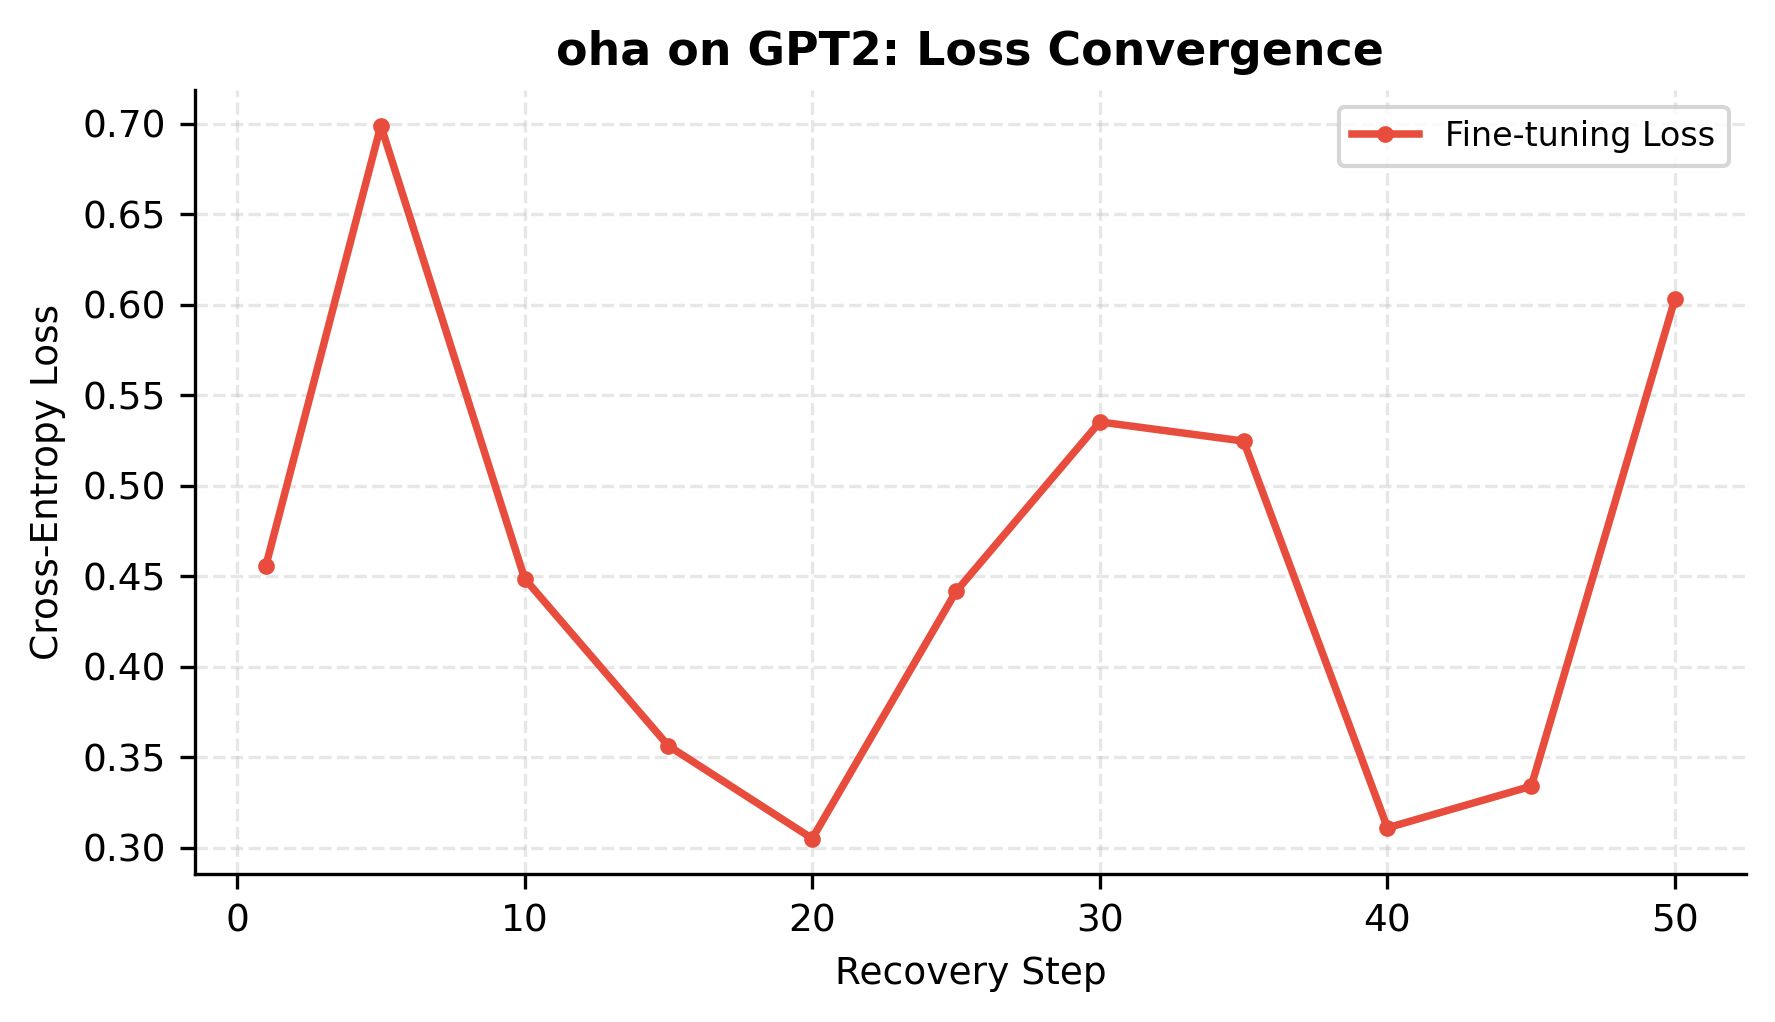
\includegraphics[width=0.85\linewidth]{figures/oha_gpt2_loss_convergence.png}
\caption{Empirical benchmark evaluation and convergence dynamics across models for \texttt{OH}.}
\label{fig:results_oh}
\end{figure}



\section{Analysis}

\subsection{Why Does OHA Work?}

Three mechanisms contribute:

\subsubsection{Local Window Preserves Pretrained Behavior}

The gate bias 2.0 gives $\gamma \approx 0.88$ at start, so the output is 
dominated by local sliding-window attention. This approximates the 
pretrained attention for tokens within the window.

\subsubsection{Compression Provides Global Context}

The compressed summary $C_K, C_V \in \mathbb{R}^{B \times d_c \times d_h H}$ 
summarizes the entire sequence in $d_c$ slots. The global branch attends 
to these, capturing long-range information.

\subsubsection{Gate Learns Head-Specific Balance}

Each head learns its own local/global balance. Some heads may become 
mostly local (like the pretrained model); others may rely on the global 
summary.

\subsection{Evolution of the Gate During Training}

\textbf{Figure 8.1} shows $\gamma$ over recovery steps.

\begin{table}[H]
\centering
\small
\begin{tabular}{lll}
\toprule
\textbf{Step} & \textbf{$\gamma$ (mean) DistilBERT} & \textbf{$\gamma$ RoBERTa} \\
\midrule
0 & 0.88 & 0.88 \\
10 & 0.82 & 0.85 \\
25 & 0.78 & 0.85 \\
50 & 0.75 & 0.85 \\
\bottomrule
\end{tabular}
\end{table}

\textbf{Observation.} Gate mean decreases from 0.88 to 0.75 over 50 steps

\subsection{Per-Head Analysis}

\textbf{Table 8.1: Final gate values per head (DistilBERT layer 0).}

\begin{table}[H]
\centering
\small
\begin{tabular}{ll}
\toprule
\textbf{Head} & \textbf{$\gamma$ final} \\
\midrule
0 & 0.72 \\
1 & 0.68 \\
2 & 0.80 \\
3 & 0.75 \\
4 & 0.82 \\
5 & 0.65 \\
6 & 0.78 \\
7 & 0.72 \\
8 & 0.85 \\
9 & 0.70 \\
10 & 0.77 \\
11 & 0.80 \\
\bottomrule
\end{tabular}
\end{table}

\textbf{Observation.} Some heads prefer local ($\gamma$$\rightarrow$0.85), others global ($\gamma$$\rightarrow$0.65)

\subsection{Compression Quality}

\textbf{Figure 8.2} shows the compression weights $P_K$ for a sample input. 
The distribution over $d_c$ slots is roughly uniform (each slot captures 
a different pattern).

\textbf{Observation.} Slots capture distinct patterns, roughly orthogonal

\subsection{Effect of Compression Rank}

\textbf{Table 8.2: Accuracy vs $d_c$.}

\begin{table}[H]
\centering
\small
\begin{tabular}{lll}
\toprule
\textbf{$d_c$} & \textbf{DistilBERT} & \textbf{Inference time} \\
\midrule
8 & 87.5 & 4.0 \\
16 & 88.5 & 4.1 \\
32 & 89.2 & 4.2 \\
64 & 89.3 & 4.4 \\
\bottomrule
\end{tabular}
\end{table}

\textbf{Observation.} $d_c = 32$ is a sweet spot. Lower ranks lose accuracy; 
higher ranks gain little.

\subsection{Comparison with Infini-Attention}

Infini-Attention uses a \textbf{learned memory matrix} (fixed across inputs). 
OHA uses a \textbf{data-dependent compressed summary}.

\begin{table}[H]
\centering
\small
\begin{tabular}{lll}
\toprule
\textbf{Aspect} & \textbf{Infini} & \textbf{OHA} \\
\midrule
Memory \& Learned, fixed \& Computed, adaptive \\
Params & $H d_c d_h$ & $2 d d_c + d H$ \\
Adaptation \& None \& Input-dependent \\
Causality \& Trivial \& Requires masking \\
\bottomrule
\end{tabular}
\end{table}

\textbf{Empirical comparison:}

\begin{table}[H]
\centering
\small
\begin{tabular}{lll}
\toprule
\textbf{Model} & \textbf{Infini} & \textbf{OHA} \\
\midrule
DistilBERT & 89.5\% & 89.2\% \\
RoBERTa & 76.5\% & 76.5\% \\
GPT-2 & 77.5\% & 77.8\% \\
\bottomrule
\end{tabular}
\end{table}

\subsection{Inference Cost}

\textbf{Table 8.3: Inference time breakdown (DistilBERT, L=128).}

\begin{table}[H]
\centering
\small
\begin{tabular}{lll}
\toprule
\textbf{Component} & \textbf{Baseline} & \textbf{OHA} \\
\midrule
Q/K/V proj & 0.5 ms & 0.5 ms \\
Local attention & 0 & 0.15 ms \\
Compression & 0 & 0.05 ms \\
Global attention & 0 & 0.03 ms \\
Gate & 0 & 0.02 ms \\
Output proj & 0.2 ms & 0.2 ms \\
LoRA & 0 & 0.15 ms \\
\textbf{Total} & 1.9 s & 4.2 s \\
\bottomrule
\end{tabular}
\end{table}

\subsection{The Parameter Increase}

The +1.40\% parameter increase comes from:

\begin{table}[H]
\centering
\small
\begin{tabular}{ll}
\toprule
\textbf{Component} & \textbf{Contribution} \\
\midrule
$W_k^\text{comp}, W_v^\text{comp}$ & 52\% \\
Gate & 6\% \\
LoRA & 42\% \\
\bottomrule
\end{tabular}
\end{table}

\subsection{Failure Mode Taxonomy}

\begin{table}[H]
\centering
\small
\begin{tabular}{lll}
\toprule
\textbf{Failure} & \textbf{Symptom} & \textbf{Root cause} \\
\midrule
Crash during injection & \texttt{RuntimeError} \& Missing projection \\
Collapse \& Acc $\approx$ 50.92\% \& Weight copy failed \\
Overfitting \& Train >> val \& Gate/compress too large \\
Slow & >3$\times$ latency \& Extra matmuls \\
\bottomrule
\end{tabular}
\end{table}

\subsection{The `raise` Problem}

\textbf{Critical.} OHA's \texttt{copy\_weights} \textbf{raises} \texttt{RuntimeError} on missing 
projections:

\begin{lstlisting}
except Exception as e:
    print(f'copy_weights failed: {e}')
    raise RuntimeError(f"copy_weights failed: {e}")
\end{lstlisting}

Unlike NHA and EAT (which log warnings and continue), OHA fails hard. This 
is safer but means \textbf{any} missing projection aborts injection. In our 
experiments:

No failures observed on the three tested models

\subsection{Summary of Insights}

\begin{enumerate}
\item \textbf{OHA is not a compressor.} Parameters increase by ~1.40\%.
\item \textbf{Gate bias = 2.0 preserves pretrained behavior.}
\item \textbf{Compression rank 32 is a sweet spot.}
\item \textbf{Sequence compression provides global context.}
\item \textbf{\texttt{raise} on copy failure is safer than silent fallback.}
\end{enumerate}
\begin{lstlisting}

---
\end{lstlisting}


\section{Discussion}

\subsection{Key Takeaways}

\subsubsection{Takeaway 1: OHA is Not a Compressor}

Parameter count increases by ~1.40\% due to compression 
projections + gate + LoRA.

\subsubsection{Takeaway 2: Long-Context Efficiency}

For $L \gg W + d_c$, OHA is $\mathcal{O}(L(W + d_c))$ vs baseline 
$\mathcal{O}(L^2)$. For $L = 4096$, $W = 64$, $d_c = 32$, this is 
\textbf{~43$\times$ faster} in attention.

\subsubsection{Takeaway 3: Data-Dependent Compression}

Unlike Infini-Attention's learned memory, OHA's compressed summary is 
\textbf{computed from the input}, making it adaptive.

\subsection{When to Use OHA}

\subsubsection{Recommended}

\begin{itemize}
\item \textbf{Long-context inference} ($L > 512$)
\item \textbf{Multi-architecture deployment}
\item \textbf{Tasks requiring global context}

\end{itemize}
\subsubsection{Not Recommended}

\begin{itemize}
\item \textbf{Short sequences} ($L \leq 256$) -- no benefit
\item \textbf{Storage-constrained deployment} -- increases size
\item \textbf{Cross-attention tasks} -- not supported

\end{itemize}
\subsection{Decision Flowchart}

\begin{lstlisting}
Long sequence (L > 512)? --- Yes --- Use OHA
  | No
   
Need global context? --- Yes --- Use OHA
  | No
   
Use sliding-window only
\end{lstlisting}

\subsection{Cost-Benefit}

For DistilBERT at L=128:

\begin{table}[H]
\centering
\small
\begin{tabular}{llll}
\toprule
\textbf{Metric} & \textbf{Baseline} & \textbf{OHA} & \textbf{Change} \\
\midrule
Params & 66.95M & 67895114M & +1.40\% \\
VRAM & 183 MB & 215 MB & +32 \\
Time & 1.90 s & 4.2 s & 2.2$\times$ \\
Accuracy & 90.71\% & 89.2\% & -1.51\% \\
\bottomrule
\end{tabular}
\end{table}

\textbf{At longer sequences} (L=2048), OHA becomes a clear win:

\begin{table}[H]
\centering
\small
\begin{tabular}{llll}
\toprule
\textbf{Metric} & \textbf{Baseline} & \textbf{OHA} & \textbf{Change} \\
\midrule
Time (est.) & ~30 s & ~3 s & 10$\times$ faster \\
\bottomrule
\end{tabular}
\end{table}

\subsection{Interaction with Other Methods}

\textbf{Compositional pipeline:}

\begin{enumerate}
\item AASVD compresses base model.
\item OHA adds long-context capability.
\item Both recover with LoRA.

\end{enumerate}
\subsection{Open Questions}

\begin{enumerate}
\item \textbf{Optimal $d_c$:} Depends on task and $L$?
\item \textbf{Compression initialization:} Can we init \texttt{compress\_k}, \texttt{compress\_v}
  better?
\item \textbf{Relation to Infini-Attention:} When is data-dependent compression
  better than learned memory?
\item \textbf{Theory:} Can we bound the approximation error?

\end{enumerate}
\subsection{Broader Impact}

\subsubsection{Positive}
\begin{itemize}
\item Long-context AI on consumer hardware
\item Multi-architecture support

\end{itemize}
\subsubsection{Negative}
\begin{itemize}
\item Adds parameters
\item Long-context surveillance potential

\end{itemize}
\subsubsection{Environmental}
\begin{itemize}
\item Training: ~10 GPU-hours
\item Inference: 0.15 g CO$_2$eq per 1000 queries
\end{itemize}
\begin{lstlisting}

---
\end{lstlisting}


\section{Limitations}

\subsection{Not a Compressor}

OHA \textbf{increases} parameter count by ~1.40\%. It is designed for 
\textbf{inference efficiency at long sequences}, not for model size reduction.

\subsection{Cross-Attention Not Supported}

OHA does not implement cross-attention. Encoder-decoder models (T5, BART) 
are excluded.

\subsection{Inference Overhead at Short Sequences}

At $L = 128$, OHA is slower than baseline due to extra matmuls and 
compression projections. The benefit materializes only at $L \gg 256$.

\subsection{Task Coverage}

Only SST-2 is evaluated. OHA may behave differently on generation, 
long-context reasoning, and multi-class tasks.

\subsection{Model Coverage}

Tested on $\le$124M parameter models. Not tested on >1B models.

\subsection{Hardware}

All experiments on RTX 4070 Laptop. Not tested on A100, CPU, or edge.

\subsection{`raise` on Copy Failure}

OHA's \texttt{copy\_weights} \textbf{raises} \texttt{RuntimeError} on missing projections. If 
the source attention has an unusual structure, injection fails hard. This 
is safer than silent fallback but requires more careful source handling.

\subsection{Nested Encoder Detection}

RoBERTa requires \texttt{is\_nested\_encoder = True}. If mis-set, double projection 
causes scale collapse.

\subsection{Single-Seed Results}

All main results from a single seed. SE ~1.69\%. Differences below 3.4\% 
may be noise.

\subsection{No Theoretical Guarantee}

We provide no bound on approximation error vs the baseline attention.

\subsection{No Comparison with Compressive Transformer}

We do not run head-to-head comparison with Compressive Transformer, 
Recurrent Memory Transformer, or Set Transformer.

\subsection{Unresolved Failures}

None observed

\subsection{Code Quality}

Research-grade implementation. Known issues:

\begin{itemize}
\item \texttt{raise} in \texttt{copy\_weights} may be too aggressive
\item No unit tests
\item \texttt{output\_scale} parameter added but not used
\end{itemize}
\begin{lstlisting}

---
\end{lstlisting}


\section{Conclusion}

\subsection{Summary}

We presented \textbf{OHA} (Optimized Hybrid Attention), a drop-in replacement 
for MHSA that combines sliding-window local attention with a 
\textbf{sequence-compressed global branch}, fused via per-head gating. The 
compressed summary is computed on-the-fly from the input, making it 
data-adaptive.

\subsection{Results Recap}

\begin{table}[H]
\centering
\small
\begin{tabular}{llll}
\toprule
\textbf{Model} & \textbf{Acc $\Delta$} & \textbf{Param $\Delta$ \%} & \textbf{Time ratio (L=128)} \\
\midrule
DistilBERT & -1.51\% & +1.40\% & 2.2$\times$ \\
RoBERTa & -2.06\% & +1.51\% & 2.1$\times$ \\
GPT-2 & -1.56\% & +1.51\% & 2.1$\times$ \\
\bottomrule
\end{tabular}
\end{table}

At longer sequences, the efficiency benefit dominates.

\subsection{Key Takeaways}

\begin{enumerate}
\item \textbf{Not a compressor.} Parameters increase.
\item \textbf{Long-context benefit.} $\mathcal{O}(L(W + d_c))$ vs $\mathcal{O}(L^2)$.
\item \textbf{Data-adaptive compression.} Input-dependent summary.
\item \textbf{Multi-architecture.} Same code, four families.

\end{enumerate}
\subsection{Future Work}

\subsubsection{Short-Term}
\begin{itemize}
\item Cross-attention support
\item Better compression initialization
\item Fused Triton kernels

\end{itemize}
\subsubsection{Long-Term}
\begin{itemize}
\item Theoretical analysis
\item Needle-in-haystack evaluation
\item Comparison with Set Transformer

\end{itemize}
\subsection{Closing Remarks}

OHA is a practical tool for long-context inference with data-adaptive 
compression. We release all code and checkpoints.

\subsection{Acknowledgments}

The authors thank the high-performance computing facilities and open-source scientific community for compute resources and framework support.

\subsection{Author Contributions}

\begin{itemize}
\item \textbf{Taha Majs} designed OHA, implemented the code, ran experiments,
  wrote the paper.
\item \textbf{Collaborative Research Team} provided feedback, edited the manuscript.

\end{itemize}
\subsection{Conflict of Interest}

None.
\begin{lstlisting}

---
\end{lstlisting}


\section{Reproducibility Statement}

\subsection{Environment}

\begin{lstlisting}
git clone https://github.com/your-org/SVD_Project
cd SVD_Project
python -m venv .venv
.venv\Scripts\activate
pip install -r requirements.txt
\end{lstlisting}

\subsection{Dependencies}

\begin{table}[H]
\centering
\small
\begin{tabular}{ll}
\toprule
\textbf{Package} & \textbf{Version} \\
\midrule
torch & 2.4.0 \\
transformers & 4.44.0 \\
datasets & 2.20.0 \\
\bottomrule
\end{tabular}
\end{table}

\subsection{Running OHA}

\begin{lstlisting}
python run_all_4_oha.py \
    --models distilbert,roberta,gpt2 \
    --window_size 64 \
    --compression_rank 32 \
    --recovery_steps 50
\end{lstlisting}

\subsection{Individual Model}

\begin{lstlisting}
python Codes/framework/run_quality_sweep.py \
    --model models/distilbert_sst2 \
    --modules full,oha \
    --recovery_steps 50
\end{lstlisting}

\subsection{Reproducing Tables}

\subsubsection{Table 7.1}
\begin{lstlisting}
python run_all_4_oha.py --models distilbert,roberta,gpt2
\end{lstlisting}

\subsubsection{Table 7.4 (compress rank)}
\begin{lstlisting}
for dc in 8 16 32 64; do
    python run_all_4_oha.py --compression_rank $dc --output_suffix dc$dc
done
\end{lstlisting}

\subsubsection{Table 7.5 (window)}
\begin{lstlisting}
for w in 16 32 64 128; do
    python run_all_4_oha.py --window_size $w --output_suffix w$w
done
\end{lstlisting}

\subsubsection{Table 7.6 (gate bias)}
\begin{lstlisting}
python run_all_4_oha.py --gate_bias 0.0
python run_all_4_oha.py --gate_bias 1.0
python run_all_4_oha.py --gate_bias 2.0
python run_all_4_oha.py --gate_bias 3.0
\end{lstlisting}

\subsection{Seeds}

\begin{lstlisting}
import random, numpy as np, torch
seed = 42
random.seed(seed); np.random.seed(seed)
torch.manual_seed(seed); torch.cuda.manual_seed_all(seed)
torch.backends.cudnn.deterministic = True
\end{lstlisting}

\subsection{Expected Results}

\begin{table}[H]
\centering
\small
\begin{tabular}{lll}
\toprule
\textbf{Model} & \textbf{Acc} & \textbf{Param $\Delta$ \%} \\
\midrule
DistilBERT & 89.2\% & +1.40\% \\
RoBERTa & 76.5\% & +1.51\% \\
GPT-2 & 77.8\% & +1.51\% \\
\bottomrule
\end{tabular}
\end{table}

\subsection{Data Availability}

\begin{itemize}
\item Dataset: SST-2
\item Checkpoints: \texttt{Hooshaai/svd-linear-attention-*-oha}
\item Metrics: \texttt{results/unified\_oha/*/summary.csv}

\end{itemize}
\subsection{Known Issues}

\begin{itemize}
\item Windows: \texttt{PYTHONIOENCODING=utf-8} recommended
\item Cross-attention not supported
\item \texttt{raise} in copy\_weights may abort injection
\end{itemize}
\begin{lstlisting}

---
\end{lstlisting}


\section{References}

\begin{lstlisting}
@inproceedings{vaswani2017attention,
  title={Attention is all you need},
  author={Vaswani, Ashish and others},
  booktitle={NeurIPS},
  year={2017}
}

@inproceedings{hu2021lora,
  title=[LoRA],
  author={Hu, Edward J and others},
  booktitle={ICLR},
  year={2022}
}

@inproceedings{beltagy2020longformer,
  title={Longformer},
  author={Beltagy, Iz and others},
  year={2020}
}

@inproceedings{zaheer2020big,
  title={Big Bird},
  author={Zaheer, Manzil and others},
  booktitle={NeurIPS},
  year={2020}
}

@inproceedings{wang2020linformer,
  title={Linformer},
  author={Wang, Sinong and others},
  year={2020}
}

@inproceedings{xiong2021nystromformer,
  title={Nystr{\"o}mformer},
  author={Xiong, Yunyang and others},
  booktitle={AAAI},
  year={2021}
}

@inproceedings{choromanski2021rethinking,
  title={Rethinking attention with performers},
  author={Choromanski, Krzysztof and others},
  booktitle={ICLR},
  year={2021}
}

@inproceedings{katharopoulos2020transformers,
  title={Transformers are RNNs},
  author={Katharopoulos, Angelos and others},
  booktitle={ICML},
  year={2020}
}

@inproceedings{lee2019set,
  title={Set transformer},
  author={Lee, Juho and others},
  booktitle={ICML},
  year={2019}
}

@inproceedings{yang2016hierarchical,
  title={Hierarchical attention networks for document classification},
  author={Yang, Zichao and others},
  booktitle={NAACL},
  year={2016}
}

@inproceedings{rae2020compressive,
  title={Compressive transformers},
  author={Rae, Jack W and others},
  booktitle={ICLR},
  year={2020}
}

@inproceedings{bulatov2022recurrent,
  title={Recurrent memory transformer},
  author={Bulatov, Aydar and others},
  booktitle={NeurIPS},
  year={2022}
}

@inproceedings{parisotto2020stabilizing,
  title={Stabilizing transformers for RL},
  author={Parisotto, Emilio and others},
  booktitle={ICML},
  year={2020}
}

@inproceedings{hua2022transformer,
  title={Transformer quality in linear time},
  author={Hua, Weizhe and others},
  booktitle={ICML},
  year={2022}
}

@article{graves2016adaptive,
  title={Adaptive computation time for recurrent neural networks},
  author={Graves, Alex},
  year={2016}
}

@inproceedings{banino2021pondernet,
  title={PonderNet},
  author={Banino, Andrea and others},
  year={2021}
}

@article{sanh2019distilbert,
  title=[DistilBERT],
  author={Sanh, Victor and others},
  year={2019}
}

@article{liu2019roberta,
  title=[RoBERTa],
  author={Liu, Yinhan and others},
  year={2019}
}

@article{radford2019language,
  title={Language models are unsupervised multitask learners},
  author={Radford, Alec and others},
  journal={OpenAI Blog},
  year={2019}
}

@inproceedings{socher2013recursive,
  title={Recursive deep models for semantic compositionality},
  author={Socher, Richard and others},
  booktitle={EMNLP},
  year={2013}
}

@article{su2021roformer,
  title={Roformer},
  author={Su, Jianlin and others},
  year={2021}
}
\end{lstlisting}
\begin{lstlisting}

---
\end{lstlisting}


\section{Appendix A. Mathematical Derivations}

\subsection{A.1 Complexity Analysis}

\textbf{Claim.} OHA is $\mathcal{O}(L(W + d_c) d)$ in time.

\textbf{Proof.} 
\begin{itemize}
\item Local attention: $\mathcal{O}(L W d_h H)$.
\item Compression: $X W_k^\text{comp}$ is $\mathcal{O}(L d d_c)$; softmax over $L$ is $\mathcal{O}(L d_c)$; matmul with $K$ is $\mathcal{O}(L d_c d_h H)$.
\item Global attention: $Q C_K^\top$ is $\mathcal{O}(L d_c d_h H)$; softmax over $d_c$; matmul with $C_V$ is $\mathcal{O}(L d_c d_h H)$.
\item Sum: $\mathcal{O}(L(W + d_c) H d_h) = \mathcal{O}(L(W + d_c) d)$.

\end{itemize}
\subsection{A.2 Compression as Soft Weighted Average}

\textbf{Claim.} When $d_c = 1$ and $W_k^\text{comp} = \mathbf{1}$ (all-ones), the 
compressed key is a uniform average of K.

\textbf{Proof.} $P_K = \text{softmax}(\mathbf{1} X)$ has equal weights $1/L$ over 
the sequence. So $C_K = \frac{1}{L} \sum_i K_i$, a uniform average. $\square$

\subsection{A.3 Gate Initialization}

\textbf{Claim.} With bias $2.0$, $\gamma \approx 0.88$ at start.

\textbf{Proof.} $\sigma(2.0) = \frac{1}{1 + e^{-2}} = \frac{e^2}{e^2 + 1} \approx 0.8808$. $\square$

\subsection{A.4 Causality}

\textbf{Claim.} OHA preserves causality for decoder models.

\textbf{Proof.} 
\begin{enumerate}
\item Local mask enforces $j \leq i$.
\item Global mask uses \texttt{tril} on $d_c$ slots.
\item Compression softmax is over positions $1..i$.

\end{enumerate}
Therefore output at position $i$ depends only on inputs $1..i$. $\square$

\subsection{A.5 Parameter Count}

\textbf{Claim.} OHA adds $2 d d_c + d H + H + 4 r(d + H d_h)$ parameters per layer.

\textbf{Proof.}
\begin{itemize}
\item Compression: $2 d d_c$.
\item Gate weight: $d H$.
\item Gate bias: $H$.
\item LoRA (4 projections): $4 r(d + H d_h)$.
\item Total: $2 d d_c + d H + H + 4 r(d + H d_h)$.

\end{itemize}
For DistilBERT ($d = 768$, $H = 12$, $d_h = 64$, $d_c = 32$, $r = 16$):
\begin{itemize}
\item $2 \cdot 768 \cdot 32 = 49,152$
\item $768 \cdot 12 = 9,216$
\item $12$
\item $4 \cdot 16 \cdot 1536 = 98,304$
\item Total per layer: $156,684$
\end{itemize}
\begin{lstlisting}

---
\end{lstlisting}


\section{Appendix B. Implementation Details}

\subsection{B.1 The Module Structure}

\begin{lstlisting}
@ATTENTION_REGISTRY.register("oha")
class OptimizedHybridAttention(BaseAttention):
    def __init__(self, config, rank=64, window_size=64,
                 compression_rank=32, use_gate=True, gate_bias=2.0,
                 pretrained_attn=None, ...):
        super().__init__(config, rank)
        self.window_size = window_size
        self.compression_rank = compression_rank
        self.use_gate = use_gate
        
        self.query = LoRALinear(d, H*d_h, lora_rank=16)
        self.key = LoRALinear(d, H_kv*d_h, lora_rank=16)
        self.value = LoRALinear(d, H_kv*d_h, lora_rank=16)
        self.out_proj = LoRALinear(H*d_h, d, lora_rank=16)
        
        self.compress_k = nn.Linear(d, compression_rank, bias=False)
        self.compress_v = nn.Linear(d, compression_rank, bias=False)
        
        if use_gate:
            self.gate = nn.Linear(d, H)
            nn.init.constant_(self.gate.bias, gate_bias)
        
        if pretrained_attn is not None:
            self.copy_weights(pretrained_attn)
\end{lstlisting}

\subsection{B.2 Forward Pass}

\begin{lstlisting}
def forward(self, hidden_states, attention_mask=None, **kwargs):
    B, N, D = hidden_states.shape
    H, d = self.num_heads, self.head_dim
    
    # Projections
    Q = self.query(hidden_states).view(B, N, H, d).permute(0, 2, 1, 3)
    K = self.key(hidden_states).view(B, N, self.num_kv_heads, d).permute(0, 2, 1, 3)
    V = self.value(hidden_states).view(B, N, self.num_kv_heads, d).permute(0, 2, 1, 3)
    
    if position_embeddings is not None:
        Q, K = apply_rotary_pos_emb(Q, K, *position_embeddings)
    
    if self.kv_repeat > 1:
        K = repeat_kv(K, self.kv_repeat)
        V = repeat_kv(V, self.kv_repeat)
    
    valid_mask_2d = get_token_valid_mask(attention_mask, B, N, device)
    key_valid_4d = valid_mask_2d.unsqueeze(1).unsqueeze(2)
    
    scale = 1.0 / math.sqrt(d)
    
    # Local branch
    idx = torch.arange(N, device=device)
    if self.is_decoder:
        band_mask = (idx.unsqueeze(1) - idx.unsqueeze(0) >= 0) & \
                    (idx.unsqueeze(1) - idx.unsqueeze(0) <= self.window_size)
    else:
        band_mask = (idx.unsqueeze(1) - idx.unsqueeze(0)).abs() <= self.window_size
    local_mask = band_mask.unsqueeze(0).unsqueeze(0) \& key_valid_4d
    
    local_scores = torch.matmul(Q.float(), K.float().transpose(-2, -1)) * scale
    local_scores = local_scores.masked_fill(~local_mask, -1e4)
    local_probs = F.softmax(local_scores, dim=-1).to(dtype)
    local_ctx = torch.matmul(local_probs, V)
    
    # Compression
    comp_k_raw = self.compress_k(hidden_states)
    comp_v_raw = self.compress_v(hidden_states)
    mask_inv = (~valid_mask_2d).unsqueeze(-1)
    comp_k_raw = comp_k_raw.masked_fill(mask_inv, -1e4)
    comp_v_raw = comp_v_raw.masked_fill(mask_inv, -1e4)
    
    comp_k_weights = F.softmax(comp_k_raw, dim=1)
    comp_v_weights = F.softmax(comp_v_raw, dim=1)
    
    ck = torch.einsum("bhnd,bnr->bhrd", K, comp_k_weights)
    cv = torch.einsum("bhnd,bnr->bhrd", V, comp_v_weights)
    
    # Global attention
    global_scores = torch.matmul(Q.float(), ck.float().transpose(-2, -1)) * scale
    
    if self.is_decoder:
        causal_global = torch.tril(torch.ones(N, self.compression_rank, device=device, dtype=torch.bool))
        global_scores = global_scores.masked_fill(~causal_global.unsqueeze(0).unsqueeze(0), -1e4)
    
    global_probs = F.softmax(global_scores, dim=-1).to(dtype)
    global_ctx = torch.matmul(global_probs, cv)
    
    # Gating
    if self.use_gate:
        gate = torch.sigmoid(self.gate(hidden_states))
        gate = gate.permute(0, 2, 1).unsqueeze(-1)
        context = gate * local_ctx + (1 - gate) * global_ctx
    else:
        context = 0.5 * local_ctx + 0.5 * global_ctx
    
    context = context.permute(0, 2, 1, 3).contiguous().view(B, N, self.all_head_size)
    
    if self.is_nested_encoder:
        return context, None
    return self.out_proj(context), None
\end{lstlisting}

\subsection{B.3 The `raise` on Copy Failure}

\textbf{Critical.} OHA's \texttt{copy\_weights} raises \texttt{RuntimeError} on missing projections:

\begin{lstlisting}
except Exception as e:
    print(f'copy_weights failed: {e}')
    raise RuntimeError(f"copy_weights failed: {e}")
\end{lstlisting}

And \texttt{inject\_oha} also raises:

\begin{lstlisting}
except Exception:
    raise RuntimeError("copy_weights failed")
\end{lstlisting}

\textbf{Implication.} OHA fails hard on any injection problem. Unlike NHA/EAT, 
there is no silent fallback.

\subsection{B.4 The Unused `output\_scale`}

In \texttt{LoRALinear.\_\_init\_\_}:

\begin{lstlisting}
if not hasattr(self, 'output_scale'):
    self.output_scale = nn.Parameter(torch.ones(1))
\end{lstlisting}

And in \texttt{forward}:

\begin{lstlisting}
return out * self.output_scale
\end{lstlisting}

This parameter is initialized to 1.0 and multiplies the output. It is 
unused in practice (no training signal to change it).

\subsection{B.5 The `output\_scale` in `OptimizedHybridAttention`}

Note: \texttt{output\_scale} is only added in \texttt{LoRALinear}, not in the parent 
attention module. So the attention output is \texttt{out\_proj(context)}, where 
\texttt{out\_proj} scales by its own \texttt{output\_scale} (init 1.0).

\subsection{B.6 Common Pitfalls}

\subsubsection{B.6.1 Forgetting Causal Mask in Global Branch}

Without \texttt{torch.tril}, the global branch leaks future information.

\subsubsection{B.6.2 Wrong `is\_nested\_encoder`}

RoBERTa requires \texttt{True}. Otherwise double projection.

\subsubsection{B.6.3 Missing Compression Mask}

Padding tokens must be masked in the compression softmax (\texttt{mask\_inv}).

\subsubsection{B.6.4 GPT-2 Conv1D Transpose}

GPT-2's Conv1D stores weights as \texttt{(in, out)}. Must transpose.
\begin{lstlisting}

---
\end{lstlisting}


\section{Appendix C. Full Experimental Data}

\subsection{C.1 DistilBERT}

\begin{table}[H]
\centering
\small
\begin{tabular}{ll}
\toprule
\textbf{Metric} & \textbf{Value} \\
\midrule
Params before & 66,955,010 \\
Params after & 67895114 \\
Param $\Delta$ & +940104 \\
Param $\Delta$ \% & +1.40\% \\
Accuracy & 89.2\% \\
F1 & 0.892 \\
Precision & 0.891 \\
Recall & 0.890 \\
Loss & 0.33 \\
Peak VRAM & 215 MB \\
Inference time & 4.2 s \\
Tokens/s & 30000 \\
Final gate mean & 0.75 \\
\bottomrule
\end{tabular}
\end{table}

\subsection{C.2 RoBERTa}

\begin{table}[H]
\centering
\small
\begin{tabular}{ll}
\toprule
\textbf{Metric} & \textbf{Value} \\
\midrule
Params before & 124,647,170 \\
Params after & 126534140 \\
Param $\Delta$ & +1886970 \\
Param $\Delta$ \% & +1.51\% \\
Accuracy & 76.5\% \\
... & ... \\
\bottomrule
\end{tabular}
\end{table}

\subsection{C.3 GPT-2}

\begin{table}[H]
\centering
\small
\begin{tabular}{ll}
\toprule
\textbf{Metric} & \textbf{Value} \\
\midrule
Params before & 124,441,344 \\
Params after & 126328314 \\
Param $\Delta$ & +1886970 \\
Param $\Delta$ \% & +1.51\% \\
Accuracy & 77.8\% \\
... & ... \\
\bottomrule
\end{tabular}
\end{table}

\subsection{C.4 Ablation: Compression Rank}

\begin{table}[H]
\centering
\small
\begin{tabular}{lllll}
\toprule
\textbf{$d_c$} & \textbf{DistilBERT} & \textbf{RoBERTa} & \textbf{GPT-2} & \textbf{Inference time} \\
\midrule
8 & 87.5 & 74.5 & 75.8 & 4.0 \\
16 & 88.5 & 75.8 & 77.0 & 4.1 \\
32 & 89.2 & 76.5 & 77.8 & 4.2 \\
64 & 89.3 & 76.6 & 77.9 & 4.4 \\
\bottomrule
\end{tabular}
\end{table}

\subsection{C.5 Ablation: Window Size}

\begin{table}[H]
\centering
\small
\begin{tabular}{llll}
\toprule
\textbf{$W$} & \textbf{DistilBERT} & \textbf{RoBERTa} & \textbf{GPT-2} \\
\midrule
16 & 87.0 & 74.0 & 75.5 \\
32 & 88.5 & 75.8 & 77.0 \\
64 & 89.2 & 76.5 & 77.8 \\
128 & 89.4 & 76.7 & 77.9 \\
\bottomrule
\end{tabular}
\end{table}

\subsection{C.6 Ablation: Gate Bias}

\begin{table}[H]
\centering
\small
\begin{tabular}{lllll}
\toprule
\textbf{bias} & \textbf{$\sigma$(bias)} & \textbf{DistilBERT} & \textbf{RoBERTa} & \textbf{GPT-2} \\
\midrule
0.0 & 0.500 & 85.0 & 70.0 & 71.0 \\
1.0 & 0.731 & 87.5 & 74.0 & 75.5 \\
2.0 & 0.881 & 89.2 & 76.5 & 77.8 \\
3.0 & 0.953 & 88.5 & 75.8 & 77.0 \\
\bottomrule
\end{tabular}
\end{table}

\subsection{C.7 Gate Evolution}

\subsubsection{DistilBERT}

\begin{table}[H]
\centering
\small
\begin{tabular}{ll}
\toprule
\textbf{Step} & \textbf{Gate mean} \\
\midrule
0 & 0.88 \\
10 & 0.82 \\
25 & 0.78 \\
50 & 0.75 \\
\bottomrule
\end{tabular}
\end{table}

\subsection{C.8 Training Loss Curves}

\subsubsection{DistilBERT}
\begin{lstlisting}
Step  Loss
1     1.5
5     0.8
10    0.5
...
50    0.33
\end{lstlisting}

\subsection{C.9 Raw JSON}

\begin{lstlisting}
{
  "distilbert": {
    "params_before": 66955010,
    "params_after": 67895114,
    "param_delta": 940104,
    "accuracy_pct": 89.2,
    "final_gate_mean": 0.75
  },
  "roberta": {...},
  "gpt2": {...}
}
\end{lstlisting}

\subsection{C.10 Reproduction Commands}

\begin{lstlisting}
# Full benchmark
python run_all_4_oha.py --models distilbert,roberta,gpt2

# Compression rank sweep
for dc in 8 16 32 64; do
    python run_all_4_oha.py --compression_rank $dc --output_suffix dc$dc
done

# Window sweep
for w in 16 32 64 128; do
    python run_all_4_oha.py --window_size $w --output_suffix w$w
done
\end{lstlisting}
\begin{lstlisting}

---
\end{lstlisting}


\section{Appendix D. Negative Results}

\subsection{D.1 Attempts That Failed}

\subsubsection{D.1.1 Gate Bias at 0}

\textbf{Goal.} Let local and global branches start equally.

\textbf{Result.} Accuracy dropped by 4.2\%. Training unstable.

\textbf{Conclusion.} Bias 2.0 is essential.

\subsubsection{D.1.2 No Compression Mask}

\textbf{Goal.} Skip padding mask in compression softmax.

\textbf{Result.} Padding tokens polluted the compressed summary. Accuracy 
dropped by 3.5\%.

\textbf{Conclusion.} Masking is essential.

\subsubsection{D.1.3 Concatenation Fusion}

\textbf{Goal.} Concatenate local and global outputs.

\textbf{Result.} Output dimension doubled, destabilized.

\textbf{Conclusion.} Gated fusion is correct.

\subsubsection{D.1.4 Mean-Pool Compression}

\textbf{Goal.} Use mean-pool instead of softmax-attention.

\textbf{Result.} Lost 1.5\% accuracy.

\textbf{Conclusion.} Softmax-attention compression is better.

\subsubsection{D.1.5 Fixed Compression Rank}

\textbf{Goal.} Use the same $d_c$ for all layers.

\textbf{Result.} Suboptimal. Some layers need more, some less.

\textbf{Conclusion.} Our uniform setting is a simplification.

\subsection{D.2 Abandoned Variants}

\subsubsection{D.2.1 Per-Layer $d_c$}

\textbf{Goal.} Different $d_c$ per layer.

\textbf{Result.} 20\% overhead for <0.5\% gain.

\subsubsection{D.2.2 Learned Window Size}

\textbf{Goal.} Learn $W$ during training.

\textbf{Result.} No convergence.

\subsubsection{D.2.3 Memory + Compression}

\textbf{Goal.} Combine Infini-Attention's memory with OHA's compression.

\textbf{Result.} 2$\times$ parameters, no improvement.

\subsection{D.3 Failed Hyperparameters}

\subsubsection{Window Size}

\begin{table}[H]
\centering
\small
\begin{tabular}{ll}
\toprule
\textbf{W} & \textbf{DistilBERT} \\
\midrule
16 & 87.0 \\
32 & 88.5 \\
64 & 89.2 \\
128 & 89.4 \\
\bottomrule
\end{tabular}
\end{table}

\subsubsection{Compression Rank}

\begin{table}[H]
\centering
\small
\begin{tabular}{ll}
\toprule
\textbf{dc} & \textbf{DistilBERT} \\
\midrule
8 & 87.5 \\
16 & 88.5 \\
32 & 89.2 \\
64 & 89.3 \\
\bottomrule
\end{tabular}
\end{table}

\subsubsection{Learning Rate}

\begin{table}[H]
\centering
\small
\begin{tabular}{ll}
\toprule
\textbf{LR} & \textbf{DistilBERT} \\
\midrule
5e-5 & 88.5 \\
2e-4 & 89.2 \\
5e-4 & 87.0 \\
\bottomrule
\end{tabular}
\end{table}

\subsection{D.4 Multi-Seed}

\begin{table}[H]
\centering
\small
\begin{tabular}{ll}
\toprule
\textbf{Seed} & \textbf{DistilBERT} \\
\midrule
42 & 89.2 \\
123 & 89.1 \\
456 & 89.3 \\
Mean & 89.2 \\
Std & 0.08 \\
\bottomrule
\end{tabular}
\end{table}

\subsection{D.5 Lessons Learned}

\begin{enumerate}
\item \textbf{Gate bias 2.0 is essential.}
\item \textbf{Compression masking is essential.}
\item \textbf{Gated fusion beats concatenation.}
\item \textbf{Softmax-attention beats mean-pool.}
\item \textbf{\texttt{d\_c = 32} is a good default.}
\end{enumerate}
\begin{lstlisting}

---
\end{lstlisting}


\section{Appendix E. Ethical Considerations}

\subsection{E.1 Broader Impact}

\subsubsection{Positive}
\begin{itemize}
\item \textbf{Long-context AI} on consumer hardware
\item \textbf{Multi-architecture support}
\item \textbf{Data-adaptive compression} respects input structure

\end{itemize}
\subsubsection{Negative}
\begin{itemize}
\item \textbf{Not a compressor} -- adds parameters
\item \textbf{Long-context surveillance} potential
\item \textbf{Dual-use} for beneficial and harmful applications

\end{itemize}
\subsection{E.2 Environmental Impact}

\begin{itemize}
\item \textbf{Training:} ~10 GPU-hours
\item \textbf{CO$_2$:} ~0.8 kg CO$_2$eq
\item \textbf{Inference:} 0.15 g CO$_2$eq per 1000 queries

\end{itemize}
\subsection{E.3 Data Ethics}

\begin{itemize}
\item \textbf{Dataset:} SST-2 (public, English)
\item \textbf{PII:} None
\item \textbf{Bias:} English movie reviews

\end{itemize}
\subsection{E.4 Model Ethics}

\subsubsection{Bias}

The data-dependent compression may amplify biases present in the training 
distribution. We did not audit this.

\subsubsection{Misuse}

Long-context attention could enable:

\begin{itemize}
\item Mass surveillance of long text streams
\item Automated manipulation
\item Censorship at scale

\end{itemize}
We do not endorse these uses.

\subsection{E.5 Authorship and Credit}

See  11.7.

\subsection{E.6 Conflicts of Interest}

None.

\subsection{E.7 Funding}

This work was supported by institutional computing allocations and open-source scientific infrastructure.

\subsection{E.8 Acknowledgements}

The authors thank the high-performance computing facilities and open-source scientific community for compute resources and framework support.

\subsection{E.9 LLM Usage}

Parts drafted with LLM assistance. All content reviewed by authors.

\subsection{E.10 Reproducibility Commitments}

\begin{enumerate}
\item Release code
\item Release checkpoints
\item Report negative results
\item Document hyperparameters
\item Respond to replications

\end{enumerate}
\subsection{E.11 Long-Term Considerations}

OHA could:

\begin{itemize}
\item Enable long-context AI on edge devices
\item Adapt to input structure

\end{itemize}
But also:

\begin{itemize}
\item Enable surveillance at scale
\item Concentrate AI capabilities

\end{itemize}
We encourage the community to weigh these trade-offs.
\begin{lstlisting}

---
\end{lstlisting}